%!TEX root = ../thesis.tex

\section{Rectangular duals}
\newcommand{\G}{\scr G}
\renewcommand{\L}{\scr L}

In this section we will introduce the rectangular dual of a graph.

\subsection{Rectangular layouts and their duals}
  We define a \emph{rectangular layout} (or simply \emph{layout}) $\L$ to be a partition of a rectangle into finitely many interiorly disjoint rectangles such that no four rectangles meet in one point.

  We say two layouts are  \emph{combinatorially equivalent} or simply \emph{equivalent} when they have the same adjacencies with the same orientation(horizontal or vertical) between their rectangles.

\subsection{Duals of rectangular layouts}
  In the \emph{dual graph} $\dualgraph{\L}$ of a layout $\L$ we represent each rectangle by a vertex and we connect two vertices by an edge exactly when their rectangles are adjacent.

  One can also consider the \emph{extended dual graph} $\extdualgraph{\L}$ of a layout $\L$. In such a graph we not only represent each rectangle by a vertex. But furthermore we also add $4$ vertices $\pN, \pE, \pS, \pW$ (so-called \emph{poles}) in the outer face, one associated to the north, east, south, west boundary segment of the outer rectangle respectively. Two vertices are then connected if their rectangles or boundary segments intersect.

  If we take the \emph{extended dual graph} of a layout and remove the $4$ vertices corresponding to the outer face we end up with the \emph{dual graph} of that layout.

  Let us note that both the dual graph and the extended dual graph of a layout $\L$ are not the same as the \emph{graph dual} of $\L$ when we view it as a graph (namely we don't represent the outer face of $\L$ by a single vertex).

\subsection{Rectangular dual}
  We have already introduced two ways to define the dual $G$ of a layout $\L$. In the reverse direction we say a layout $\L$ is a \emph{rectangular dual} of a certain graph $G$ if we have that $G = \dualgraph{\L}$.

  A triangulation of the $k$-gon $\G$ does not necessarily have a rectangular dual nor is this dual necessarily unique. The requirements for existence are given in Theorem \ref{th:rect:exsitenceREctangularDual}. To see that a rectangular  dual is not necisicairly unique one can simply consder the two non-equivalent duals of the same graph given in Figures \ref{fig:rect:segmentdefs} and \ref{fig:rect:vertonesided}.



\subsection{Different kinds of rectangular layouts}
  We can pose different restriction on a rectangular layout $\L$. For all these restrictions we have that if they hold for one layout $\L$ they hold for all equivalent layouts.

  We will call $\L$ \emph{area-equivalent} if no matter the areas we assign to the rectangles of $\L$ there is a equivalent layout $\L'$ such that each rectangle has the assigned area.

  All other restrictions we introduce here will consider the \emph{maximal line segments} (or simply \emph{maximal segements}) of $\L$. A \emph{line segment} (or simply \emph{segment}) of $\L$ is a sequence of consecutive inner boundary segments forming a line. Such a segment is called maximal if it's not contained in any other line segment. \fxnote*{Is this neccesary?}{This notion is also introduced in \cite{Eppstein2012}}.
  A segment is \emph{one-sided} if it is on the boundary of a single rectangle. We call it \emph{$k$-sideded} if on one of the sides it is the boundary of at most $k$ rectangles. Finally, a line segment is \emph{$(k,l)$-sided} with $k<l$ if the line segment is on the boundary of at most $k$ different rectangles on one side and at most $l$ different rectangles on the other side.

  Consider for example Figure \ref{fig:rect:segmentdefs}. The three highlighted lines are all line segments. However only the red and blue segment are maximal segments. The red segment is one-sided and $(1,5)$-sided. The blue segment is $2$-sided and $(2,3)$-sided.

  \begin{figure}[h]
    \centering
    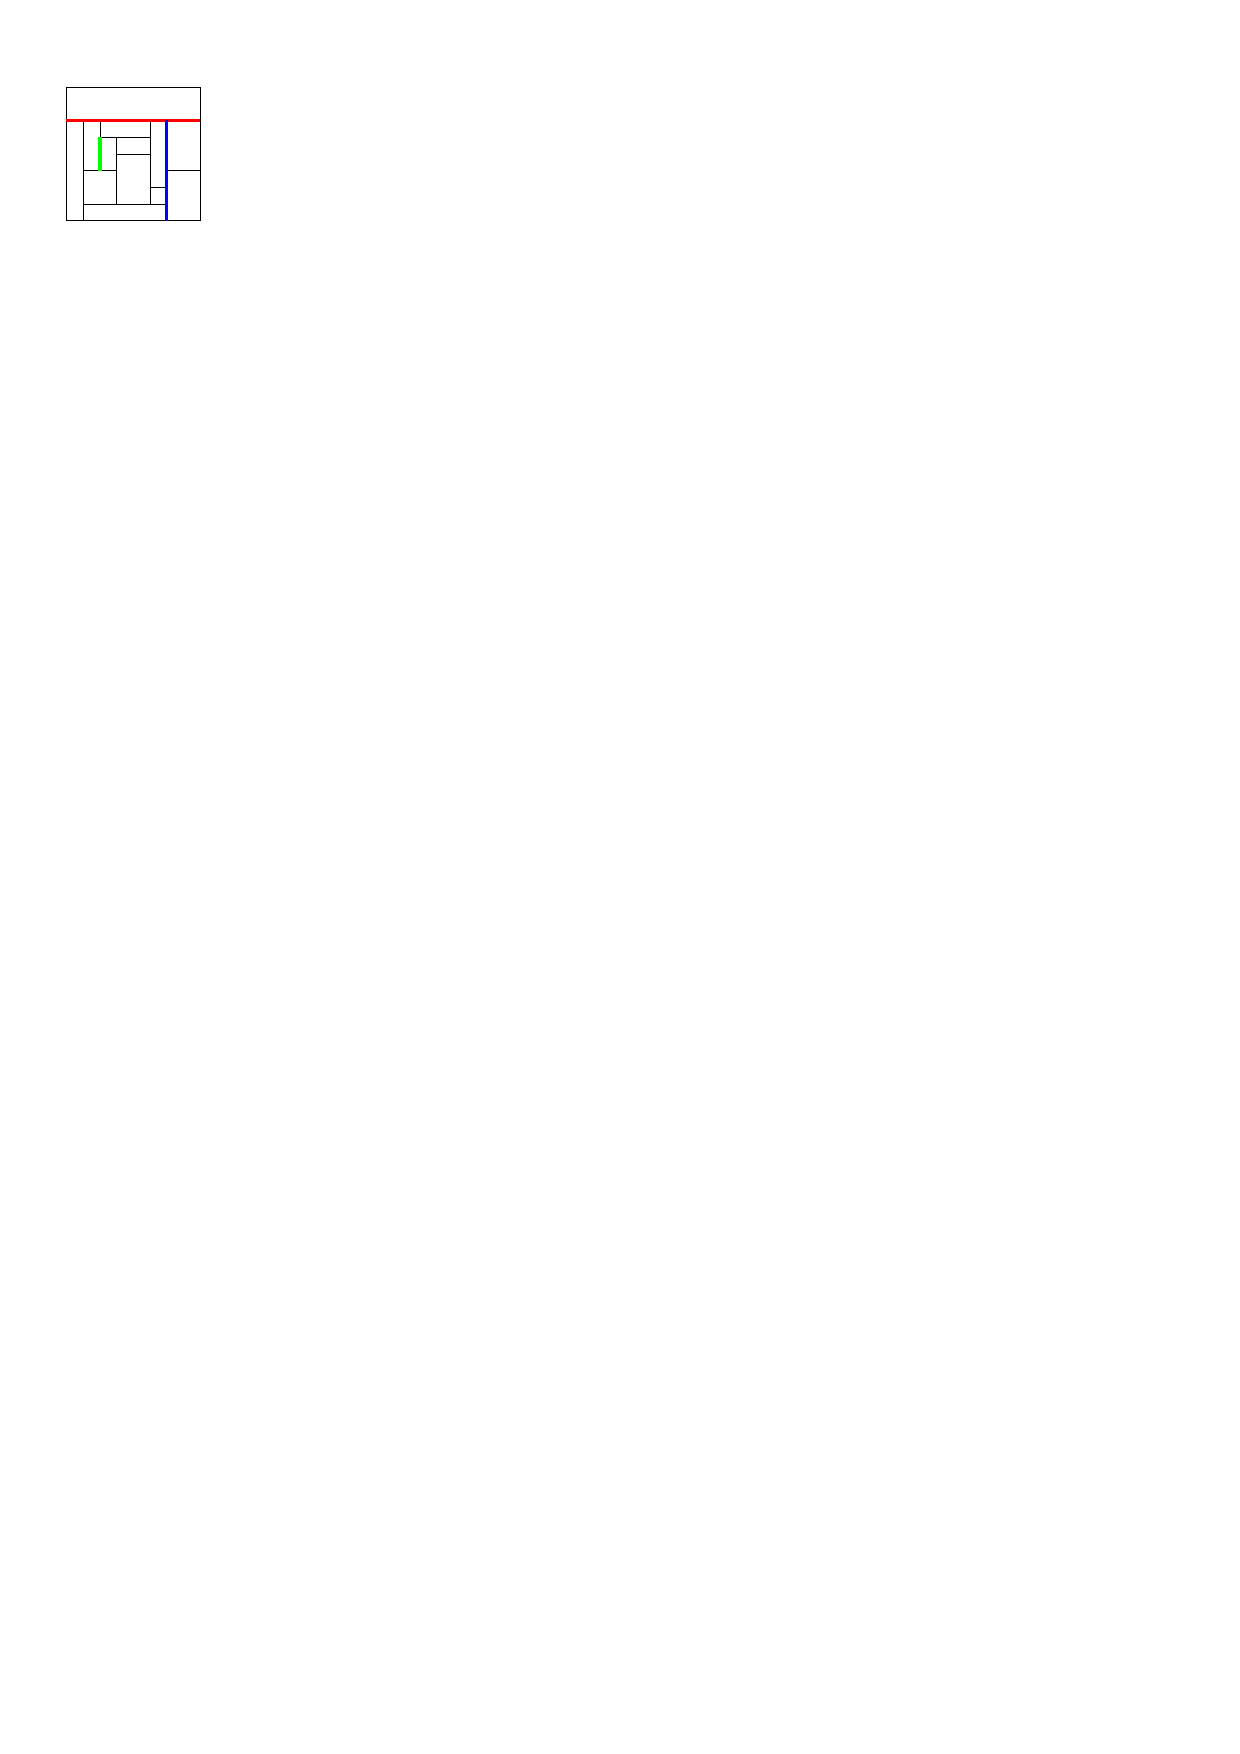
\includegraphics[scale=1]{rectangularDuals/img/segmentdefs}
    \caption{Rectangular layout with three highlighted segments}
    \label{fig:rect:segmentdefs}
  \end{figure}

  \fxwarning{Think about removing defi for $(k,l)$ sideds, this will proc a rewrite}

  We will then call a layout \emph{one-sided} if all maximal segments are one-sided. Furthermore it is called \emph{vertically one-sided} or \emph{horizontally one-sided} if just all vertical or horizontal maximal segments are one-sided. Furthermore a layout is \emph{$k$-sided} if all maximal line segments are $k$-sided and \emph{$(k,l)$-sided}  if all maximal line segments are $(k,l)$-sided.

  Consider  Figure \ref{fig:rect:vertonesided}. In this Figure a vertically one-sided rectangular layout is depicted. This layout is also $4$-sided and $(4,5)$-sided.
  \begin{figure}[h]
    \centering
    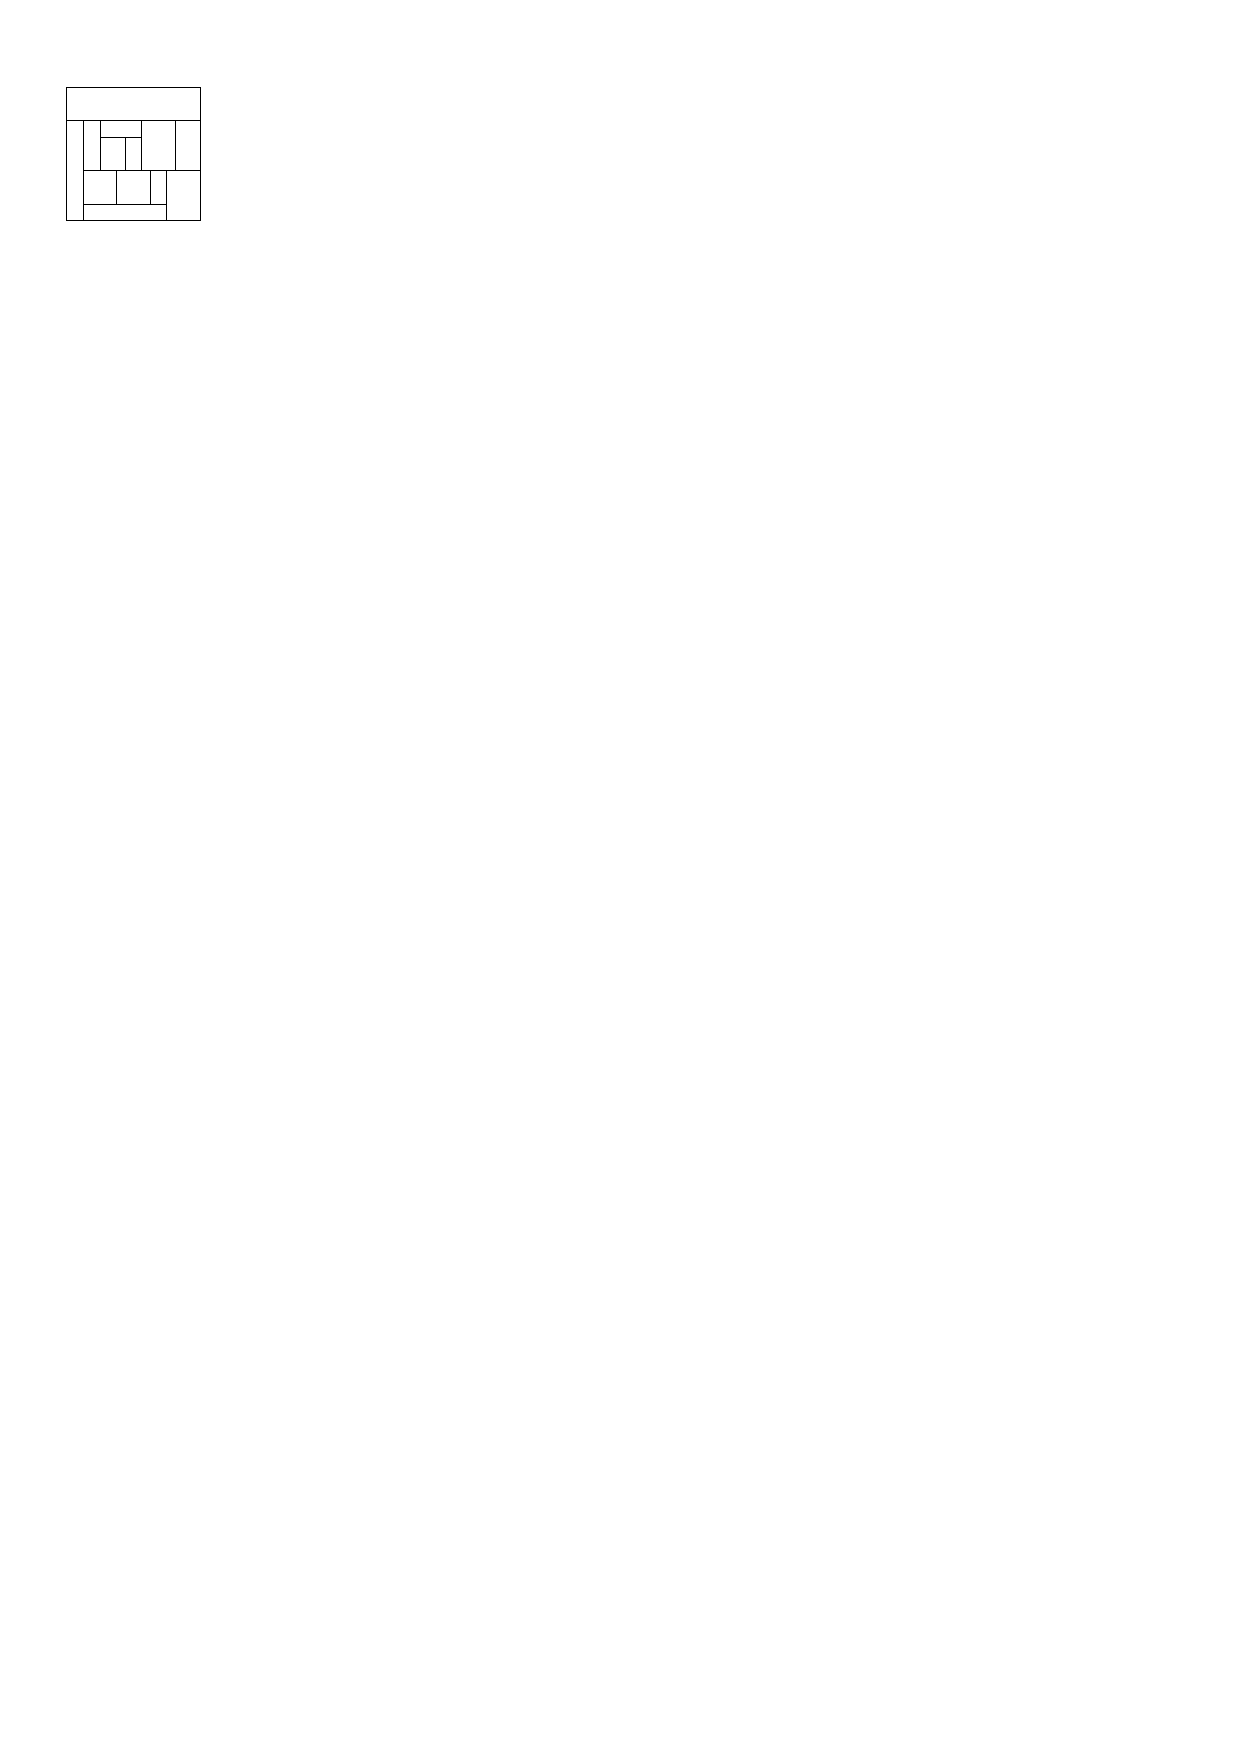
\includegraphics[scale=1]{rectangularDuals/img/vertonesided}
    \caption{A vertically one-sided rectangular layout}
    \label{fig:rect:vertonesided}
  \end{figure}

  Eppstein et al. \cite{Eppstein2012} show that a layout is area-universal if and only if it is one-sided.

\subsection{Regualar edge labeling}
  The extended dual of a layout allows a natural coloring and orientation of its edges. This \emph{regular edge labeling} can be found in the following way:
  For every edge $vw$ in $\extdualgraph{\L}$ we consider whether the shared boundary of the rectangles is vertical or horizontal we then color the edge blue or red respectively. In the first case we orient the edge from the  leftmost point to the rightmost point and in the second case we orient from bottom to top. We don't color or orient the edges between the poles.

  From the nature of the adjacencies in a rectangular layout we can deduce the following two rules for a regular edge labeling.
  \begin{enumerate}
    \item (Interior vertex) In the rotation around every interior vertex we have the following subsequent non-empty sets: Incoming red edges, incoming blue edges, outgoing red edges and outgoing blue edges. And only these sets.
    \item (Pole) $\pN$ has only incoming red edge, $\pE$ has only incoming blue edges, $\pS$ has only outgoing red edges and $\pW$ has only outgoing blue edges. Except for, of course, the uncolored edges between poles.
  \end{enumerate}

  Regular edge labeling were first introduced by Kant and He \cite{Kant1997} and were also used in \cite{Eppstein2012}. Fusy also studied these structures \cite{Fusy2006,Fusy2009} but he calls them \emph{transeversal structures}.

  He showed \cite{He1993} that given a regular edge labeling we can reconstruct a rectangular layout giving this regular edge labeling.

  A regular edge labeling  of $\ext G$ corresponds to a equivalence class of rectangular layouts $\L$ that are a rectangular dual of $G$.

  Note that we have no monocolored directed cycles because such a cycle would for example correspond to a  group of adjacent rectangles that have  no leftmost or topmost one. This is clearly absurd.

  \begin{lemma}
    \label{lm:rel:noMonoColoredTriangles}
    A regular edge labeling doesn't admit a monocolored triangle
  \end{lemma}

  \begin{proof}
    Suppose we have a monocolored triangle. Without loss of generality we will suppose that the color of this triangle is blue. Then at least one of the vertices has an incoming blue edge followed directly by an outgoing blue edge or an outgoing blue edge followed directly by an incoming blue edge in it's rotation. Thus this vertex has either an empty set of outgoing or incoming red edges, offending the coloring requirements of a REL
  \end{proof}

  \subsubsection{$st$-planar graphs}
    Kant and He \cite[pp.179]{Kant1997} show that an regular edge labeling is closely linked to a pair of $st$-planar graphs. As can be seen in Theorem \ref{th:rel:stPlanarGraphs} below.

    A $st$-planar graph is an oriented planar graph with one source (indegree 0) $s$ and one sink (outdegree 0) $t$. Both $s$ and $t$ lie on the outer face. Moreover, such a $st$-planar graph has no directed cycles.

    \begin{thrm}
      \label{th:rel:stPlanarGraphs}
      The blue edges of $G\sm{\pN,\pS}$ form a $st$-planar graph with $s= \pW$ and $t=\pE$. Moreover the red edges of $G\sm{\pW,\pE}$ form a $st$-planar graph with $s= \pS$ and $t= \pN$.
    \end{thrm}
    \begin{proof}
      Kant and He propose to add an edge and orient the outer cycle. This is necessary because they require $s$ and $t$ to be adjacent. Moreover they don't a priori require such an graph to be without directed cycles.

      A trivial adaptation of \cite[pp.179]{Kant1997} then gives us the theorem. We note that we can't get any directed cycles since a regular edge labeling has no monocolored directed cycles.
      \fxnote{We might write our own proof.}
    \end{proof}

    We will refer to these $st$-planar graphs as the \emph{blue graph} and \emph{red graph} of some regular edge labeling. We will then refer to the faces of these graphs as \emph{blue faces} and \emph{red faces}.

    Every face $F$ in an $st$-planar graph has the same structure. The boundary of $F$ consists of two directed paths with common origin $\spl(F)$ and  destination $\mrg(F)$.\fxnote{We might want to prove this.}
    These boundary paths are adjacent in the orientation at $\spl(F)$. We will say the first path in the rotation, starting at the beginning of the adjacent pair, is the \emph{right boundary path} or \emph{bottom boundary path} of $F$ and the second one is the \emph{left boundary path} or \emph{top boundary path}.

    \subsubsection{Fans}
    We introduce some more concepts to describe the interior of a blue (or red) face. Every interior edge of this face goes from one fence to the other (otherwise it's start or end vertex would offend the interior vertex condition).\fxnote{This could be a useful result in the section about cycles and their interiors.} To better understand the structure of such a strip we will describe the edges from $\spl(F)$ to $\mrg(F)$ .

    Let $u_0 , u_1, \ldots u_n$ be the vertices of the upper boundary path of $F$ and $v_0, v_1, \ldots, v_m$ the vertices of the bottom boundary path. That is $u_0=v_0 = \spl(F)$ and $u_n = v_m = \mrg(F)$. Since our graph is a triangulation $u_1v_1$ must be an edge. For the second edge in the face we have two options $u_1v_2$ or $u_2v_1$, otherwise this edge and the previous one would not form a triangle. This principle holds for every subsequent edge, we can either increase a the index of the upper boundary path or the index of the bottom boundary path. In other words, this face is a so-called \emph{triangle strip}.

    We will call a maximal sequence of at least two edges increasing the index on the bottom boundary path (and thus keeping the index on the upper path fixed) a \emph{Bottom-fan} or simply \emph{B-fan} and a maximal sequence of at least two edges increasing the index on the upper boundary path will be called a \emph{Top-fan} or just \emph{T-fan}. The \emph{size} of such a fan is the number of edges contained in the sequence. By the definition of a fan it has size of at least $2$.
    We will simply use \emph{fans} to refer to both these \emph{types} of fans (i.e. T- and B-fans).

    We will call a fan of size $3$ or larger a \emph{large fan}. Then it is only natural that we call a fan of size $2$ a \emph{small fan}.

    In a strip we alternately encounter B- and T-fans. Since if we would have two adjacent fans of the same type we would just have a single larger fan of that type.
    In Figure \ref{fig:uni:fans} we see a strip consisting of subsequently a B-fan of size $3$, a T-fan of size 2, a B-fan of size $2$, a T-fan of size $6$, a B-fan of size $3$ and a T-fan of size $3$.

    \begin{figure}[h]
      \centering
      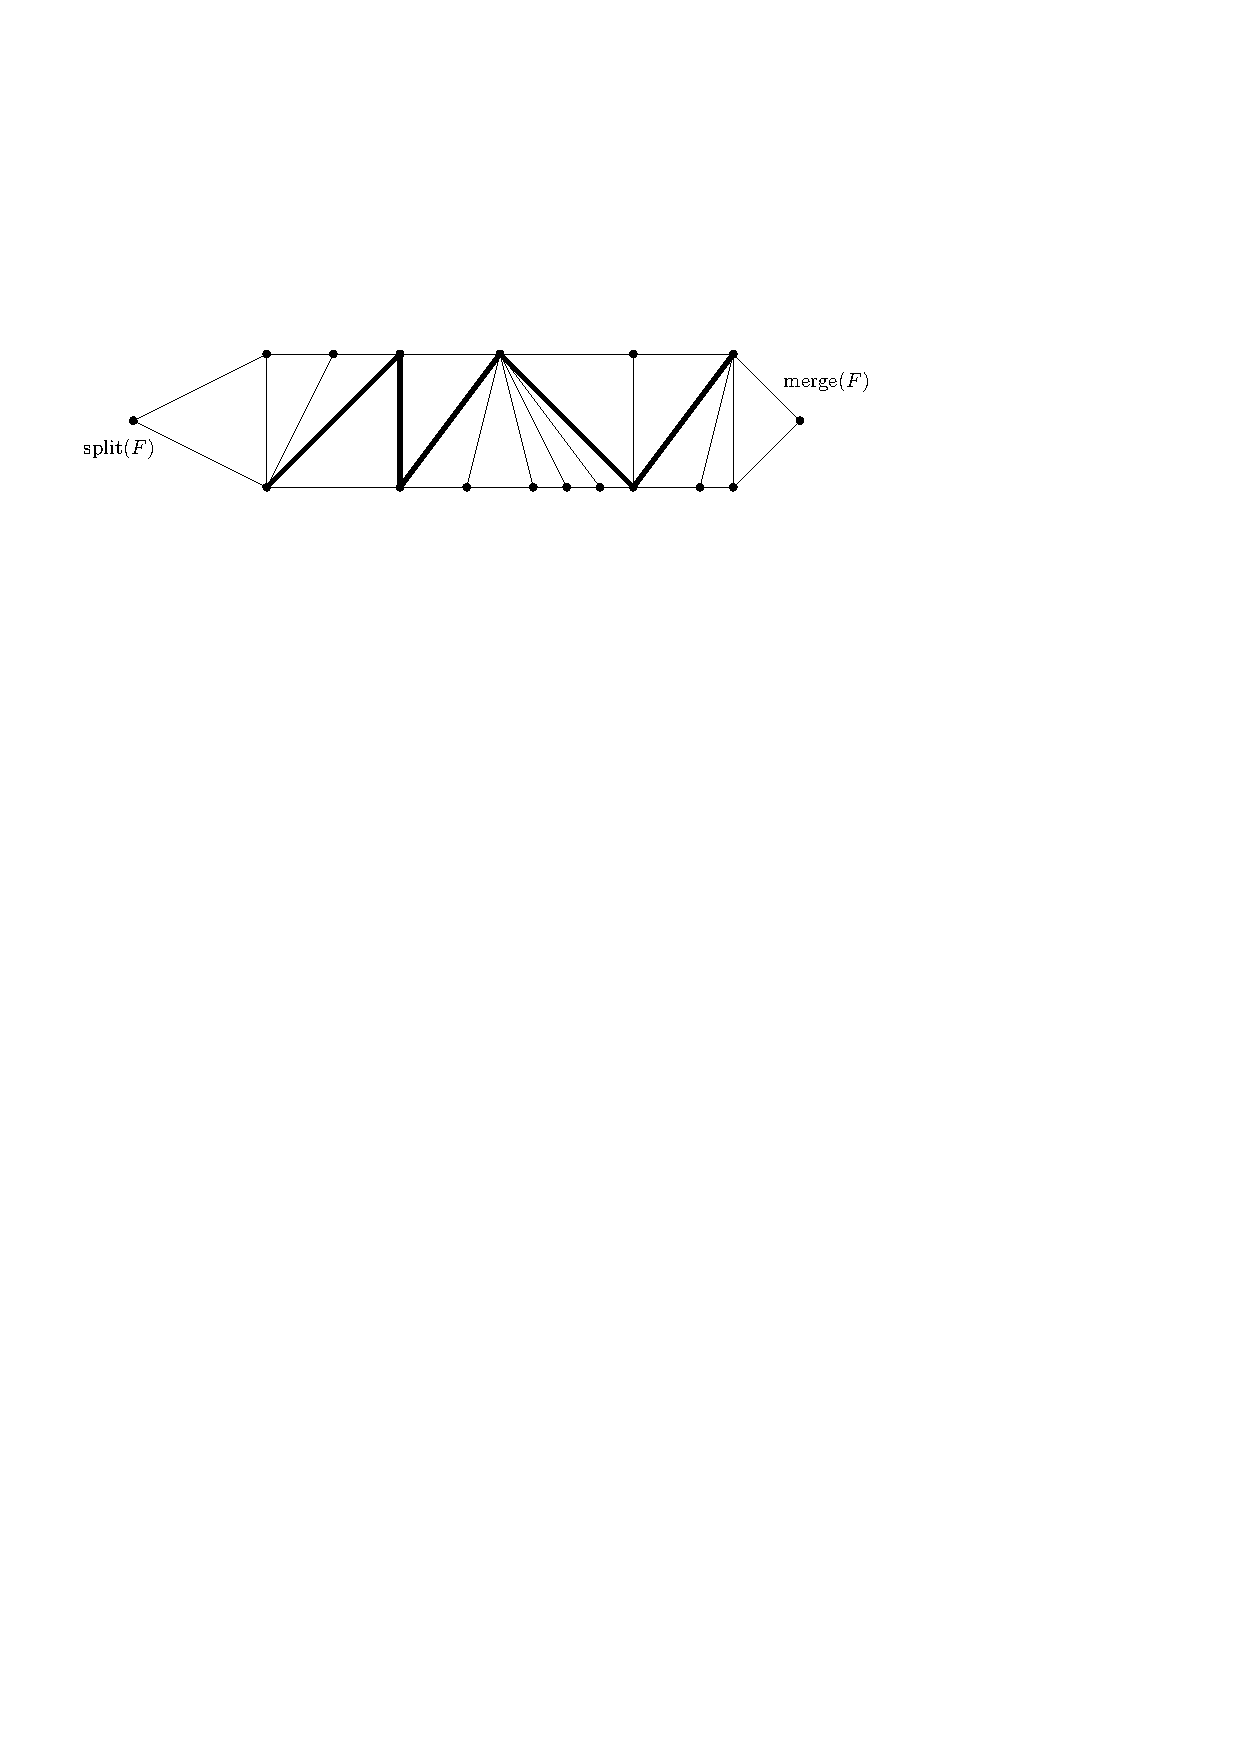
\includegraphics[scale=.9]{rectangularDuals/img/fans}
      \caption{}
      \label{fig:uni:fans}
    \end{figure}


   We introduce some more terminology for fans: \emph{outer edges}, \emph{fan handles} and the \emph{rim} as can be seen in Figure \ref{fig:rect:fanTerms}. The \emph{fan handle} is the vertex shared by all edges in the fan. The \emph{rim} is the path between the vertices of each edge that is not the fan handle. The \emph{outer rim} are the two extreme edges of this path and the \emph{outer edges} are the edges between the fan handles and the extreme vertices of the \emph{rim}.

   \begin{figure}[h]
     \centering
     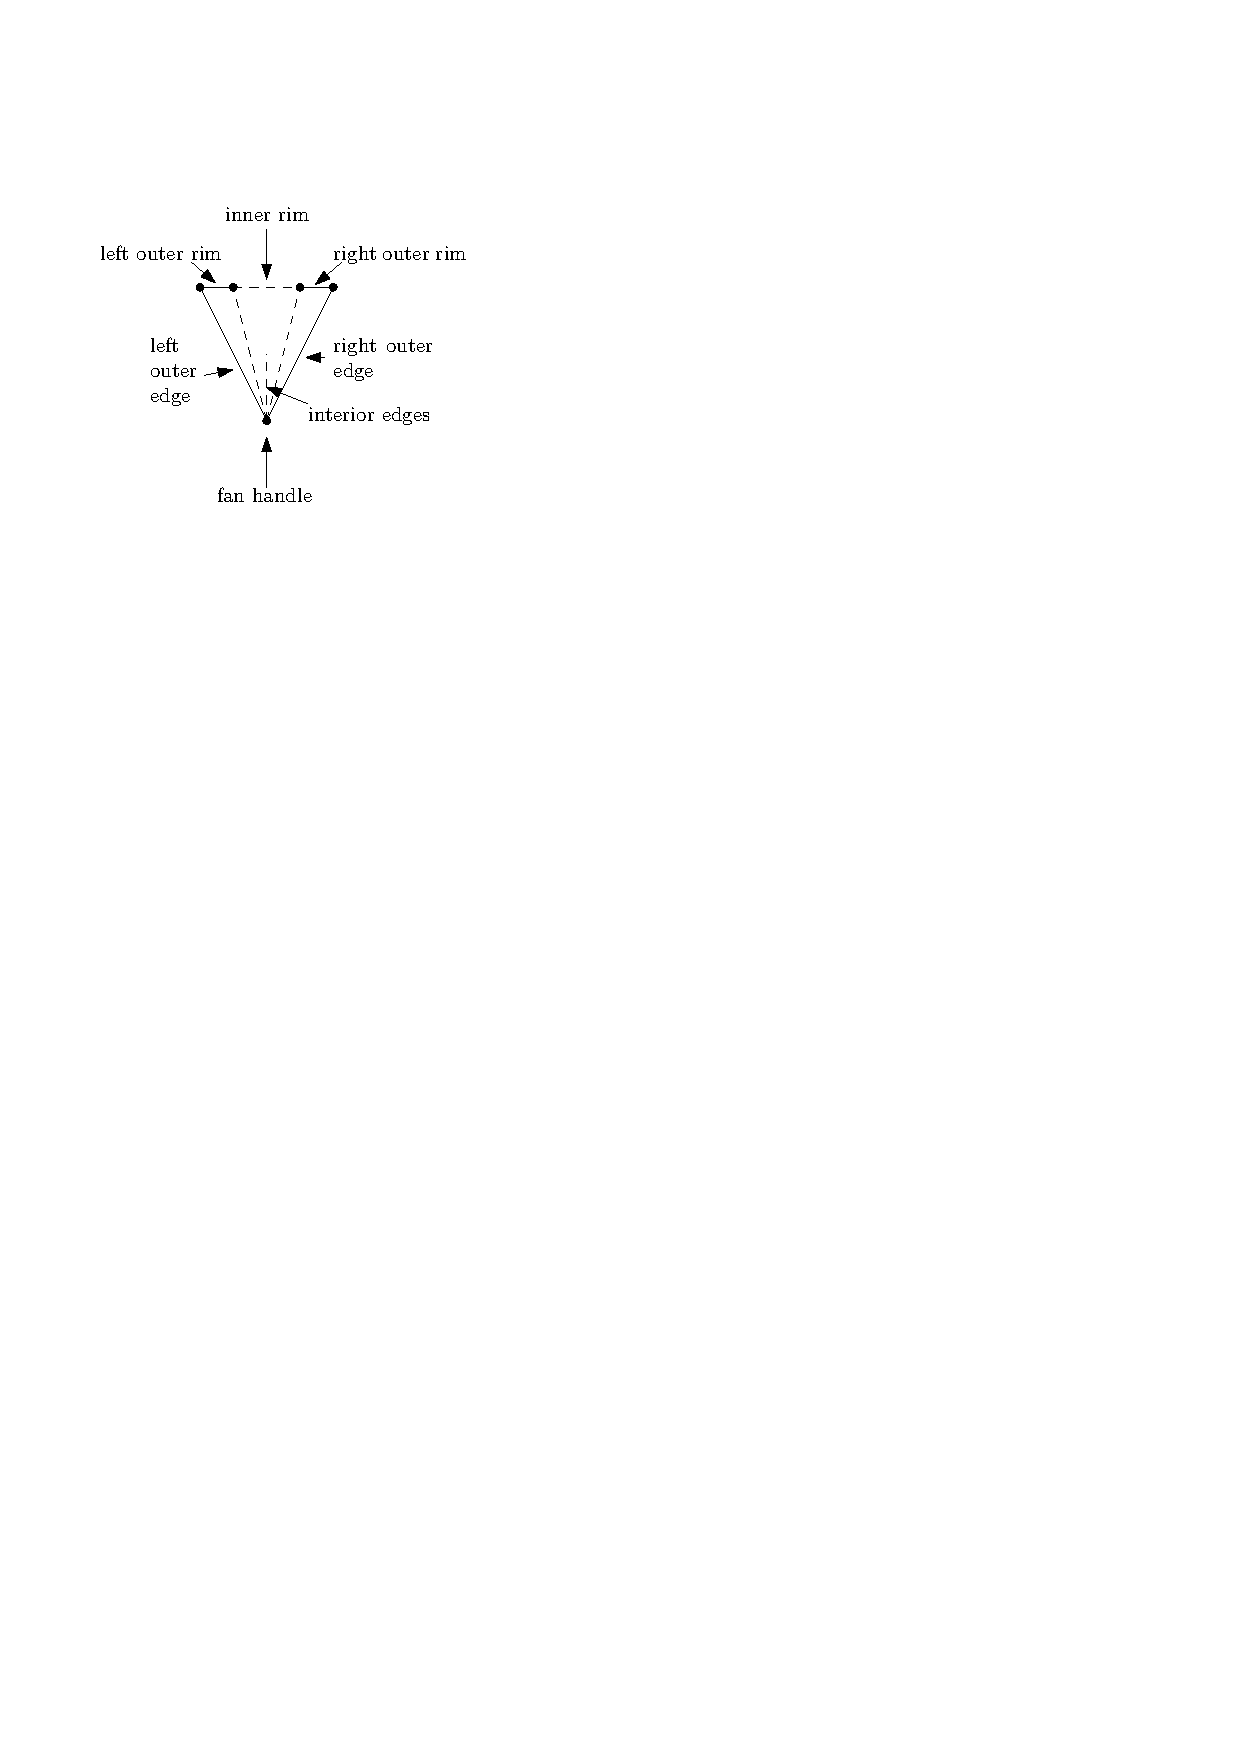
\includegraphics[scale=1]{rectangularDuals/img/fanterms}
     \caption{}
     \label{fig:rect:fanTerms}
   \end{figure}

  \subsubsection{Regular edge labellings and maximal segments}
    From the way that we color a \rel for a given layout $\L$ we can see in Figure \ref{fig:rect:relSegmentFace} that a horizontal maximal segment leads to a blue face and a vertical maximal segment leads to a red face.

    \begin{figure}[h]
      \centering
      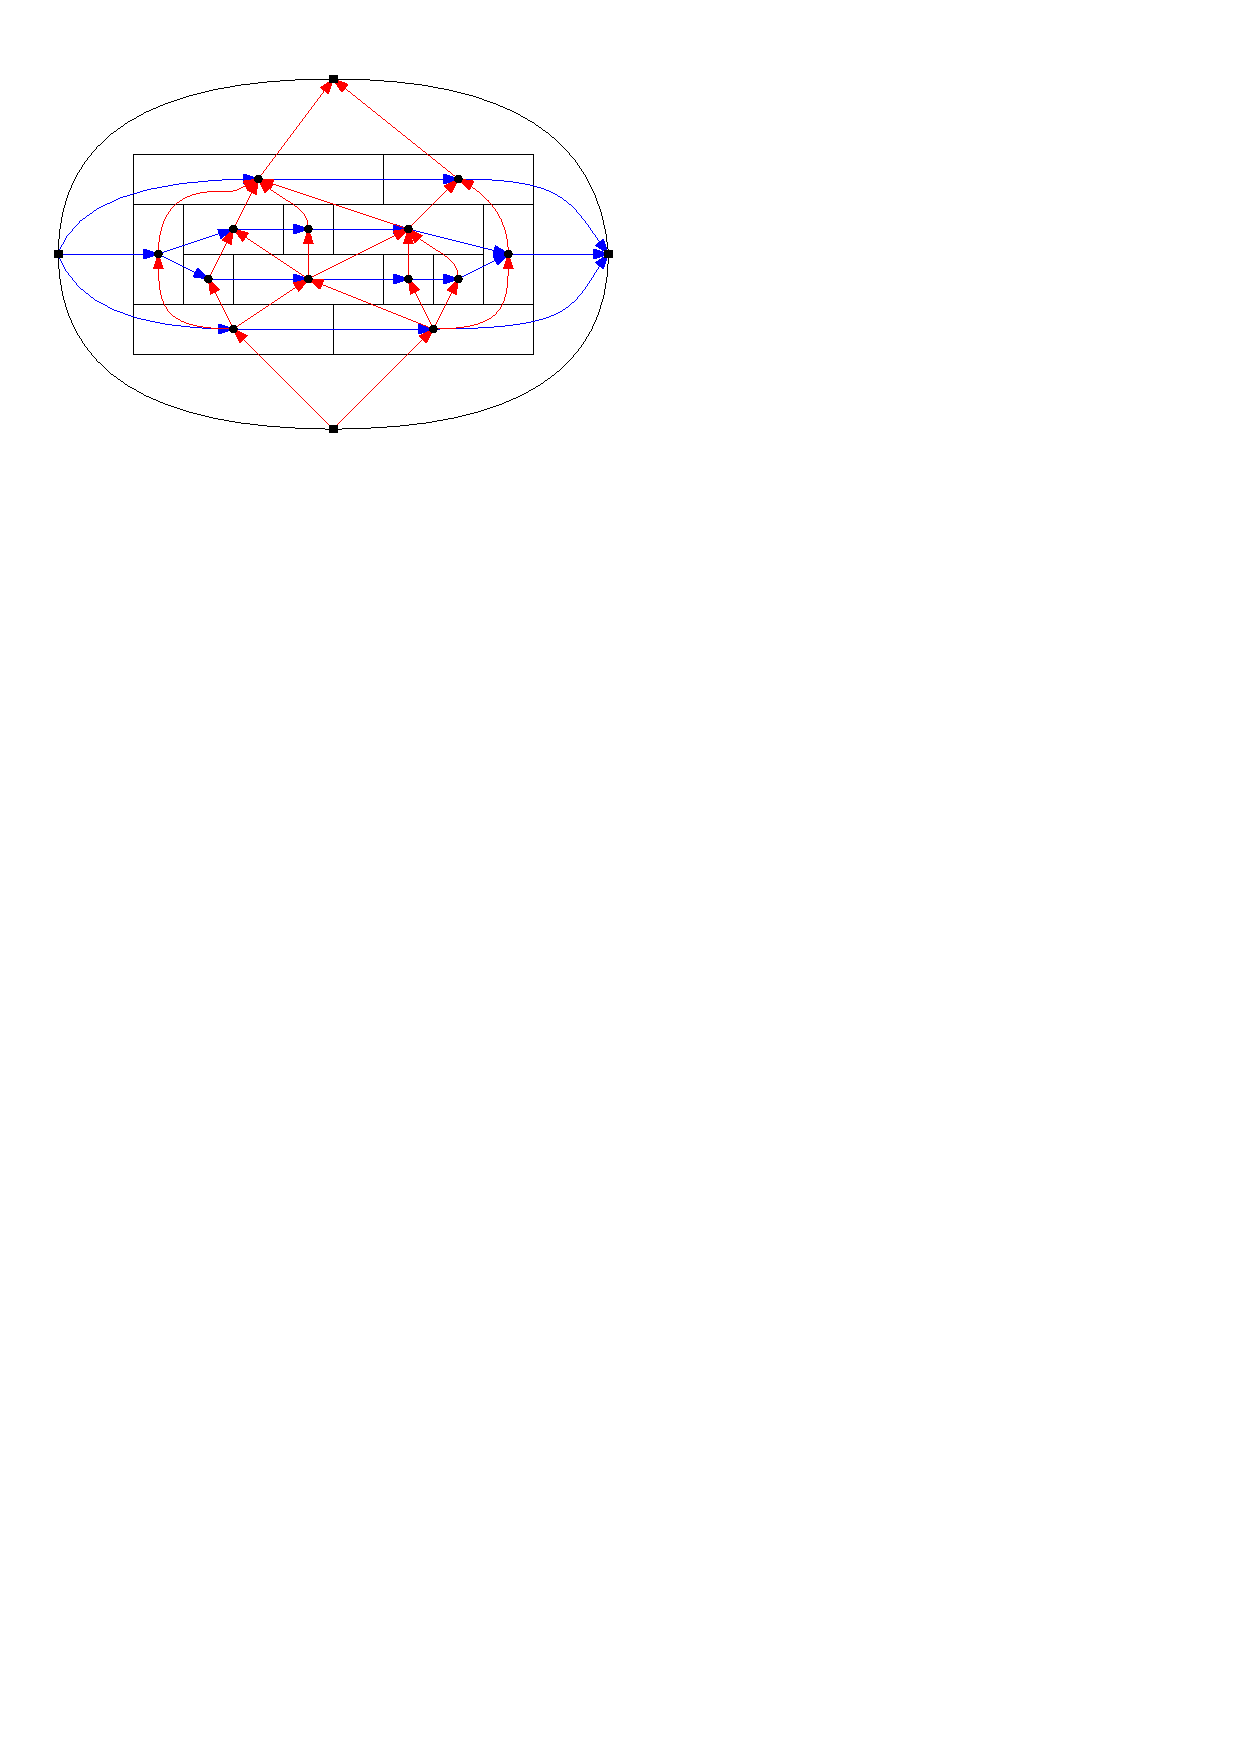
\includegraphics[scale=1]{rectangularDuals/img/relSegmentFaceRescale}
      \caption{}
      \label{fig:rect:relSegmentFace}
    \end{figure}

    For either type of maximal segment we denote the corresponding face with $F$. The number of interior vertices of both boundary paths without $\mrg(F)$ and $\spl(F)$ is the number of rectangles on the respective sides of the maximal segment.

    Hence a one-sided maximal segment corresponds to a face with one boundary path of length $2$\footnote{A boundary path can't have length $1$ since by construction of a \rel it encloses a maximal segment and thus has to go trough at least one intermediate rectangle/vertex.}. And a $(k,l)$-sided maximal segment has a short boundary path of length at most $k+1$ and a longer boundary path of length at most $l+1$\footnote{Recall that the length of a path its edgecount.}.
    We will for the ease of the discussion ofter refer to such a face as an $(k,l)$-face.

\subsection{Corner assignments}
  \fxnote[inline, nomargin]{might want to move this to the next section}

  Given a layout $\L$ we can thus easily find the (extended) dual. However finding a rectangular dual of a plane triangulated graph $G$ is more involved. Due to the algorithm by He \cite{He1993} this boils down to finding a regular edge labeling of $G$ with $4$ additional vertices $\pN, \pE, \pS, \pW$. We will define $G$ and these $4$ additional vertices to be a \emph{corner assignment} of $G$.

  \begin{defi}[Corner assignment]
    A \emph{corner assignment} $\ext G$ of $G$ is a augmentation of $G$ with $4$ vertices (which we will call it's \emph{poles}). Such that
    \begin{enumerate}
    \item every interior face has degree $3$ and the exterior face has degree $4$.
    \item all poles are incident to the outer face
    \end{enumerate}
  \end{defi}

  We have the following result due to Kozminski and Kinnen

  \begin{thrm}[Existence of a rectangular dual]
    \label{th:rect:exsitenceREctangularDual}
    A plane triangulated graph $\G$ has a rectangular dual if and only if it has an corner assignment without separating triangles $\ext \G$
  \end{thrm}

  \begin{proof}
    This shown independently in \cite{Kozminski1984} and  \cite{Ungar1953}
  \end{proof}

  Due to this theorem we will call a corner assignment without separating triangles a valid corner assignment.

  A graph with a valid corner assignment $G$ can have more then one valid corner assignment. Each such corner assignment fixes which of the rectangles are in the corners of the rectangular dual $\L$.

  Note that a graph $G$ with a separating triangle can't have any valid corner assignment, since every possible corner assignment will have a separating triangle.

  \subsubsection{Adjecent vertices and chords}
  We will call a vertex \emph{$\pS$-adjecent} when it is adjacent to $\pS$ in the current corner assignment. In the same way we will call a chord or $2$-chord \emph{$\pE$-bound}, \emph{$\pW$-bound} or \emph{polebound} when it is adjacent to $\pE$, $\pW$ or any pole respectively.
